\documentclass[10pt]{article}

% required packages
\usepackage{graphicx}
\usepackage[hidelinks]{hyperref}
\usepackage{fancyhdr}

% margins
\setlength{\headwidth}{6.40in}
\pagestyle{fancy}
\addtolength{\textwidth}{1in}
\addtolength{\textheight}{1in}
\addtolength{\evensidemargin}{0.5in}
\addtolength{\oddsidemargin}{-0.5in}
\addtolength{\topmargin}{-0.5in}


% page headers
\fancyhead{} 
\fancyhead[LO,LE]{CSE 250B}
\fancyhead[RO,RE]{Project 1}



\title{Logistic Regression with L$_2$ Regularization}

\author{Adrian Guthals (aguthals@cs.ucsd.edu),\\
David Larson (dplarson@ucsd.edu),\\
Jason Yao (j6yao@ucsd.edu)\\
\\
CSE 250B: Project \#1 \\
University of California, San Diego \\
}


\begin{document}

\maketitle


\begin{abstract}
Logistic Regression with L$_2$ Regularization is analyzed as a classification learning method for data sets with real-valued features and binary labels. Stochastic Gradient Descent (SGD) and Limited-memory BFGS (L-BFGS) are used to find the regression parameters such that the Log Conditional Likelihood (LCL) is maximized. The methods are applied to two data sets: USPS-N (images of hand-written digits) and Web (statistics on HTML web pages). Logistic regression with SGD had a higher test error percentage than L-BFGS for both the USPS-N (5.32$\pm$3.23\% vs 3.21$\pm$0.9\%) and Web data sets (8.75$\pm$4.3\% vs 5.45$\pm$1.4\%). These results support choosing L-BFGS over SGD by default for Logistic Regression. However, since L-BFGS more precisely maximizes LCL, care should be taken to prevent overfitting.
\end{abstract}



%-----------------------------------------------------------------------------
% INTRODUCTION
%-----------------------------------------------------------------------------
\section{Introduction}
\label{sec:intro}

Machine Learning (ML) is a sub-discipline of Artificial Intelligence (AI) that focuses on the development and analysis of methods that produce models from data. An often referenced example application of ML is email spam filtering, but there is a wide variety of real-world problems where ML has been successful used, from object detection using a Microsoft Kinect sensor \cite{Kinect} to forecasting of power output from a photovoltaic solar farm \cite{solar}.

ML algorithms are plentiful in number, but some are more suitable than others depending on the type of problem. Logistic regression is a ML algorithm well-suited to problems involving a set of real-valued inputs and a binary (Bernoulli) output. A real-world example of such a problem is whether a baseball player will hit a home run based on a collection of statistics (e.g. batting average, height, weight). The statistics are the real-valued inputs, whether he hits a home run is the binary output (1=yes, 0=no), and the probability of whether a player hits a home run is the determined using logistic regression. 

In this paper we analyze logistic regression's capability for classification learning using a previously study as a baseline \cite{t-logistic}. Aside from recreating the previous study's results, we also extend their work to comparing two gradient-based optimization methods for use in conjuction with the logistic regression: Stochastic Gradient Descent (SGD) and Limited-memory Broyden-Fletcher-Goldfarb-Shannon (L-BFGS).



%-----------------------------------------------------------------------------
% DESIGN OF ALGORITHMS
%-----------------------------------------------------------------------------
\section{Design and Analysis of Algorithms}
\label{sec:algorithms}

Stochastic Gradient Descent (SGD) and Limited-memory Broyden-Fletcher-Goldfarb-Shannon (L-BFGS) were each implemented in Matlab to maximize the total conditional log likelihood of each training data set. In brief, SGD incorporated a fixed learning rate $\lambda$ to control the change in log likelihood, which was averaged over random mini-batches of size $\kappa$. To control over-fitting, logistic regression was used and change in the objective function was evaluated on a random subset of size $\gamma$. Convergence was reached when change in the objective function was less than $\omega$. Our L-BFGS implementation used the the minFunc \cite{minFunc} software package to converge on the maximum likelihood with the supplied objective (Eq. \ref{LBFGS_obj}) and gradient functions (Eq. \ref{LBFGS_grad}).

For each of these algorithms, the input training data is formatted as a set of $n$ examples $x_i \ldots x_n$ where each $x_j$ is a real-valued vector of $d$ features. Each $x_i$ is correlated to a binary (Bernoulli) outcome $y_i$ by a global parameter vector $\beta$ of length $d+1$. We assume this correlation follows the model below where $x_{i0}=1$ for all $i$:

\begin{equation}\label{p}
    p_i = p(y_i|x_i;\beta) = \frac{1}{1+\exp-(\sum_{j=0}^{d} \beta_j\,x_{ij})}
\end{equation}



\subsection{SGD} 
Our SGD implementation first randomized the order of input examples to avoid repeated computation of random numbers and selected a subset of examples $x_1 \ldots x_{\gamma}$ for checking convergence of the objective function. Then sequential mini-batches of size $\kappa < n$ taken from the training set were used to update the parameter vector $\beta$ (initialized to all zero values) by the following equation. The constant $\mu$ quantifies the trade-off between maximizing likelihood and minimizing parameter values for $L_2$ Regularization.

\begin{equation}\label{SGD_grad}
    \beta := \beta + \lambda [-2 \mu \beta + \frac{1}{\kappa}\sum_{i=1}^{\kappa}{(y_i - p_i)\,x_i}]
\end{equation}

After each update of $\beta$, absolute change in the objective $\widehat{\beta}$ was computed over a constant subset of examples with the following function:

\begin{equation}\label{SGD_obj}
    \widehat{\beta} = \mu \|\beta\|^2 - \sum_{i=1}^{\gamma}{\log(p_i^{y_i}(1 - p_i)^{1-y_i})}
\end{equation}
where $\|\beta\|^2$ is the vector norm of the parameters.


Convergence was reached when change in the objective was less than $\omega$. With this configuration, the time to run the SGD is $O(\kappa\,d + \gamma\,d)$ per iteration and can be sufficiently less than $O(nd)$ (for large datasets) when $\kappa$ and $\gamma$ are properly set. If the training set is small enough to allow one epoch per iteration, one can set $\kappa = \gamma = n$ to yield a running time  of $O(nd)$.


\subsection{L-BFGS}
L-BFGS is a quasi-Newton optimization method used to find local extrema. It approximates the Hessian matrix of second derivatives using rank-one updates of the first derivatives and uses these gradients to converge on the set of hyperparameters that yield a first-order gradient of zero. minFunc is a popular Matlab implementation of L-BFGS (among other methods) that was also used in \cite{t-logistic}. To recreate the results in \cite{t-logistic}, we supplied minFunc with the following objective and gradient functions:
\begin{equation}\label{LBFGS_grad}
    \frac{\partial}{\partial \beta_j}LCL = \mu \|\beta\|^2 - \sum_{i=1}^{n}{(y_i - p_i)\,x_i}
\end{equation}

\begin{equation}\label{LBFGS_obj}
    LCL = -2 \mu \beta - \sum_{i=1}^{n}{\log(p_i^{y_i}(1 - p_i)^{1-y_i})}
\end{equation}
as well as an initial $\beta$ vector of zero values. Convergence was reached when change in the objective was less than $\omega$.



%-----------------------------------------------------------------------------
% DESIGN OF EXPERIMENTS
%-----------------------------------------------------------------------------
\section{Design of Experiments}
\label{sec:experiments}

Logistic regression models from SGD and L-BFGS were separately trained on the Web and USPS-N datasets mentioned in \cite{t-logistic}. For USPS-N, we only trained prediction models for digit 9 vs. all others. All $x_{ij}$ feature values were normalized to $[0,1]$ and all $y_i$ were converted to binary values (0/1). 30\% of each dataset was randomly selected and separated out as a validation set and the remaining 70\% was used for 10-fold cross validation. The optimal parameters $\lambda, \kappa, \gamma, \mu$ for SGD and $\mu$ for L-BFGS were chosen by grid search over the parameter space $\{10^{-4},10^{-3},...,10^{3}\}$ and observing the prediction accuracy over the validation set. Certain parameter combinations for SGD that increased the running time to over 30 minutes (on a Quad-Core 3.2 GHz CPU with 32 Gb RAM) were omitted. Although each dataset was small enough to set $\kappa$ and $\gamma$ equal to $n$ for SGD convergence, we chose to set them to $10^{3}$ to limit the time required to run SGD repeatedly for 10-fold cross validation. The convergence criterion $\omega$ was set to $10^{-4}$ as in \cite{t-logistic}. Since L-BFGS uses the objective gradient to automatically update $\lambda$, we allowed minFunc to use the default initial $\lambda_0 = 1$. The following table details the hyperparameters that were learned for each data set.

\begin{table}[htb!]
%\small
%\footnotesize
\centering
\begin{tabular}{lcccccc}
& \multicolumn{4}{c}{SGD} & & L-BFGS\\
\cline{2-5}
\cline{7-7}
 & $\lambda$ & $\kappa$ & $\gamma$ & $\mu$ & & $\mu$\\
USPS-N & $10^{-1}$ & $10^{3}$ & $10^{3}$ & $10^{-4}$ & & $10^{0}$\\
Web & $10^{-1}$ & $10^{3}$ & $10^{3}$ & $10^{-4}$ & & $10^{0}$\\
\end{tabular}
\caption{Hyperparameters of the SGD and L-BFGS methods for both data sets.}
\end{table}



%-----------------------------------------------------------------------------
% RESULTS OF EXPERIMENTS
%-----------------------------------------------------------------------------
\section{Results of Experiments}
\label{sec:results}

Figure \ref{fig:test_error} shows that logistic regression with SGD had a higher test error percentage than L-BFGS for both the USPS-N (5.32$\pm$3.23\% vs 3.21$\pm$0.9\%) and Web data sets (8.75$\pm$4.3\% vs 5.45$\pm$1.4\%). These results are reasonable considering that SGD only takes in a random subset of examples at a time and updates the parameters according to the subset. Thus, even when the SGD converges according to criteria, the overall objective function may or may not be reach the local extrema. The L-BFGS method is more thorough than SGD as it updates the parameters based on the entire training set. L-BFGS also considers the second derivative of the parameter functions in addition to the gradient.   

\begin{figure}[h]
\begin{center}
    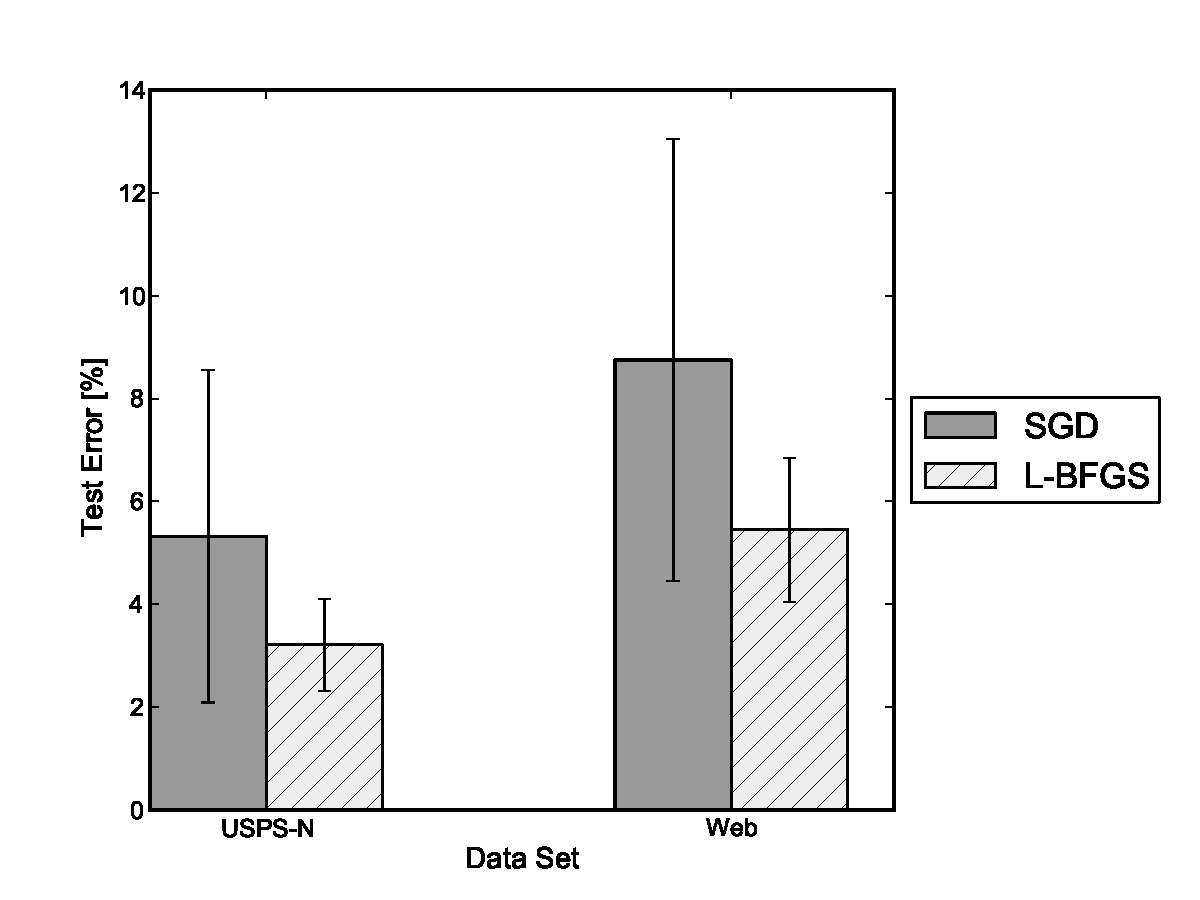
\includegraphics[width=1.0\textwidth]{test_error.pdf}
    \caption{Comparison of test error percentage for SGD (gray solid) and L-BFGS (white hatched), where the error bars are $\pm$ one standard deviation.}
    \label{fig:test_error}
\end{center}
\end{figure}



%-----------------------------------------------------------------------------
% FINDINGS AND LESSONS LEARNED
%-----------------------------------------------------------------------------
\section{Findings and Lessons Learned}
\label{sec:conclusion}

The issue of overfitting was especially relevant when training with L-BFGS. For all $\mu \leq 10^{-3}$, resulting $\beta$ parameters yielded extremely low error ($<$ 1\%) on the training data but infinite error on the validation set. Inspection of the $\beta$ values showed that they were extremely high in magnitude ($\pm 30$) compared to SGD-trained $\beta$ parameters ($\pm 2$). It was only after applying higher $\mu$ values that the magnitude of $\beta$ parameters was sufficiently reduced to yield appropriate cross-validated error. This suggests that training with L-BFGS should only be done with some regularization (we performed $L_2$ Regularization) and cross-validation of the trained models to protect against overfitting.

Although the simplified form of SGD uses minibatches of size 1, we found that larger minibatches better approxmated the true gradient and led to tighter convergence (lower T-error). In developing the SGD algorithm it also became evident that convergence was reached much faster when the set of $\gamma$ examples used to evaluate change in the objective function was constant over all iterations. At first we used the same minibatch of $\kappa$ examples (that was used to approximate the gradient) to also approximate change in the objective function. Although larger minibatches better approximate the objective, disjoint minibatchs never yield the exact same objective given the same set of $\beta$ parameters. Thus, the algorithm could not converge on a single set of optimum $\beta$ parameters as iterations progressed because it would frequently jump from one maximum to another. Although this approach failed to make use of all the training data for evaluating the objective, it allowed for tighter convergence around some local maximum without scanning all training data in each iteration. It is important to mention that 10-fold cross validation helped protect against over-fitting to a single $\gamma$-size subset because $\beta$ parameters were averaged over multiple executions of SGD (examples were randomly re-ordered prior to each training run).



%-----------------------------------------------------------------------------
% BIBLIOGRAPHY
%-----------------------------------------------------------------------------
\bibliographystyle{IEEEtran}
\bibliography{sources}


\end{document}
